\documentclass[a4paper, 11pt, titlepage]{article}
\usepackage{fancyhdr}
\usepackage{graphicx}
\usepackage{imakeidx}
\usepackage{makeidx}
\usepackage{mathtools}
\usepackage[spanish]{babel}
\usepackage{eurosym}
\usepackage{hyperref}
\usepackage{amssymb}
\usepackage{listings}
\usepackage{xcolor}
\usepackage{mathtools}
\usepackage{blkarray, bigstrut}
\usepackage{stackrel} 

\title{Estructura de computadores}
\author{Francisco Javier Balón Aguilar}

\begin{document}

\maketitle
\renewcommand{\contentsname}{Índice}
\tableofcontents
\newpage

\section{Unidad Central de Proceso (CPU)}\label{cpu}

    \subsection{Máquina de Von Neumann}

        La máquina de Von Neumann (1945) es un modelo computacional teórico referencia para 
        el diseño de arquitecturas de ordenadores.

        El modelo propone una unidad central de proceso (véase sección \ref{cpu}), que controla y gobierna la lógica 
        de la máquina, una memoria (véase sección \ref{memoria}) que contendrá instrucciones y datos, una unidad de entrada
        y salida (véase sección \ref{entradasalida}) que gestionará las entradas y salida de resultados, y un conjunto de periféricos.

        \begin{figure}[htp]
            \centering
            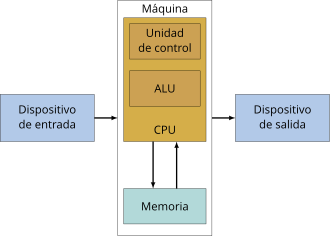
\includegraphics[width=0.7\textwidth]{resources/vonneumann.png}
            \caption{Diagrama del modelo de arquitectura Von Neumann.}
            \label{vonneumann}
        \end{figure}

        El modelo presentado, se orienta al
        procesado de información, requiriendo dos elementos: los datos y la lógica a aplicar 
        con ellos.

        Como características generales de todas las máquinas basadas en el modelo de Von Neumann, 
        podríamos citar:

        \begin{itemize}
            \item Uso de componentes lógicos básicos, tal y como puertas lógicas, transistores... 
            \item Configuración de uso general de funciones lógico-aritméticas.
            \item Uso de memoria, tanto para el almacenamiento de datos como de instrucciones.
            \item Uso de circuito secuencial (unidad de control). Véase la sección \ref{unidadcontrol} 
            para mayor detalle.
            \item Provisión de instrucciones y datos.
        \end{itemize}

        Tal y como se observa en la figura \ref{vonneumann}, los elementos que lo componen son:

        \subsubsection{Memoria en la máquina de Von Neumann}

            La memoria está compuesta por un conjunto de celdas de la misma longitud (mismo número de
            bits), que almacenan tanto datos como instrucciones, siendo cada una de ellas identificada 
            una dirección unívoca (dirección de memoria). El sistema puede leer la información contenida 
            en ellas y escribir nuevos datos.

        \subsubsection{Unidad aritmético-lógica (ALU) en la máquina de Von Neumann}

            En esta unidad se realizan las operaciones básicas lógicas y de tipo aritmético, 
            tales como sumar, restar, AND, OR, XOR...

            Los datos se obtienen de la memoria principal y se escriben en la misma los resultados 
            finales. Los resultados intermedios se almacenan temporalmente en registros de la propia 
            ALU.

        \subsubsection{Unidad de Control (UC) en la máquina de Von Neumann}

            Es la encargada de ejecutar las instrucciones almacenadas en memoria, procediendo previamente 
            a su captura y decodificación para después interpretando el tipo de instrucción a ejecutar y 
            generando posteriormente las señales de control para su interpretación.
            
        \subsubsection{Unidad de Entrada y Salida en la máquina de Von Neumann}

            Se encarga de gestionarla transferencia de información entre los periféricos y la unidad 
            central de proceso.

        \subsubsection{Buses en la máquina de Von Neumann}

            Son los elementos que interconectan los componentes. Su objetivo es por tanto la transferencia 
            de información, bien sean datos o señales entre los diferentes dispositivos.

            Por lo general distinguimos tres tipos de buses:

            \begin{itemize}
                \item \textbf{Buses de datos}.
                \item \textbf{Buses de control}.
                \item \textbf{Buses de direcciones}.
            \end{itemize}

    \subsection{Ciclo Básico de Instrucciones}

        \subsubsection{Registros y operaciones básicas}

        \subsubsection{Instrucciones, operaciones y órdenes}

        \subsubsection{Tipo de instrucciones}

    \subsection{La Unidad de Control}\label{unidadcontrol}

    \subsection{Unidad Aritmético-Lógica}

    \subsection{Modos de direccionamiento}

\section{Memoria}\label{memoria}
\section{Módulo de Entrada y Salida}\label{entradasalida}
\section{Buses}

\end{document}